\section{Honest negatives (A6)}
\label{sec:study3}
\label{sec:A6}

The studies above establish what the knowledge matrix \emph{is} --- a
function-determined object with an exact displacement accounting. This
section reports, with equal prominence, three places where it does
\emph{not} buy what one might hope. The scope of each negative is
deliberately narrow: knowledge matrices are insufficient \emph{as
invariants for the specific tasks tested here}, which is not the claim
that they are worse for every downstream use. We include these results
because they discipline the paper's claims; a canonical-representation
argument that reported only its successes would be the weaker for it.

\subsection{Adversarial detection: penultimate features win the bake-off}
\label{sec:study3-bakeoff}

\paragraph{Why it matters.}
The original version of this work proposed the knowledge matrix as the
input to an adversarial-example detector. Settling that comparison against
standard baselines is a matter of integrity: it is the v1 claim the
reviewers asked us to test, and reporting its outcome --- whatever it is
--- is what lets the rest of the paper be read at face value.

\paragraph{Setup and procedure.}
Across a $6$-detector $\times$ $3$-representation bake-off:
\begin{enumerate}
\item Fix three representations of each sample --- penultimate features,
the knowledge matrix, and logits.
\item Fix six off-the-shelf detector configurations.
\item For each (representation, detector) pair, fit the detector to
separate clean from adversarial samples and score it.
\item Count, per detector, which representation wins.
\end{enumerate}

\paragraph{Result.}
\emph{Penultimate features win $5$ of the $6$ detector configurations};
the knowledge matrix does not provide a detection advantage on this task.
We therefore \emph{withdraw the adversarial detection claim entirely} and
report the bake-off as an honest negative. We keep it prominent rather
than relegating it to an appendix: a canonical-representation argument that
reported only its successes would be the weaker for it.

\paragraph{Reading.}
This negative is consistent with the theory rather than in tension with
it. Detection asks which representation best separates two finite
empirical samples under a chosen classifier; it is a statistical-power
question about a particular discriminator, and nothing in
function-determination (Theorem~\ref{thm:maxinv}) or in the displacement
decomposition (Theorem~\ref{thm:pyth}) predicts that the canonical
representation should also be the most \emph{separable} one for an
off-the-shelf detector. What the theory does buy --- invariance under
the function-stabiliser, exact row-sum accounting, alignment-free
cross-architecture comparison --- is orthogonal to detection performance.
The honest reading is that the knowledge matrix is the right object for
the canonical-representation questions of Studies~1--3 and the wrong
object for this detector bake-off, and we say so plainly.

\subsection{Single-region LP-counterfactual: $0/54$}
\label{sec:study3-lp}

\paragraph{Why it matters.}
A second hope was that the linearisation $\Weff(x)$ underlying the
knowledge matrix could be turned into a clean, matrix-direction
counterfactual: the minimum input change that the local linear model
predicts will flip the class. Reporting that this fails --- and exactly
why --- disciplines the claim structure of the whole paper, since the same
within-region geometry (Theorem~\ref{thm:within}) that powers Study~2
predicts that a matrix direction need not transfer across region walls. It
cannot, on pretrained ImageNet networks, and the failure is structural.

\paragraph{Construction.}
For a source class $s$ and target class $t\neq s$, the
\emph{LP-counterfactual direction} at $x$ is the $\ell_1$-minimum input
perturbation $\delta\in\R^d$ that, \emph{within the linearisation around
$x$}, pushes the target--source logit gap past a margin $m>0$:
\begin{equation}
\min_{\delta} \|\delta\|_1
\quad\text{s.t.}\quad
\big(\Weff(x)_{t,\cdot}-\Weff(x)_{s,\cdot}\big)\cdot\delta
\;\ge\;
m-(f(x)_t-f(x)_s),
\label{eq:lp-cf}
\end{equation}
subject to a per-coordinate box $\delta_i\in[-x^{\text{px}}_i/\sigma_c,
(1-x^{\text{px}}_i)/\sigma_c]$ that keeps the pixel-space image in
$[0,1]$ ($x^{\text{px}}_i=x_i\sigma_c+\mu_c$ recovers the pixel
intensity from the ImageNet-normalised input). Without the box the LP is
solved in closed form by the single most cost-effective coordinate
($k=\arg\max_i|c_i|$ for $c=\Weff(x)_{t,\cdot}-\Weff(x)_{s,\cdot}$);
with the box it becomes a saturation greedy that fills coordinates in
order of $|c_i|$ until the margin is met. Both are $O(n\log n)$; the
greedy's $\ell_1$-optimality is proved in the supplementary
(cost-per-unit-swing $1/|c_i|$ is independent of the per-coordinate
bound).

\paragraph{Setup and result.}
For each architecture in $\{$ResNet-152, DenseNet-121, GoogLeNet$\}$ we
run $3$ source images $\times\,3$ source classes $\times\,2$ target
classes ($18$ LPs per architecture, $54$ in all) with margin $m=0.1$,
and for each we record a Boolean \texttt{region\_ok} flag --- True only
when $x$ and $x+\delta$ realise identical activation patterns at every
ReLU and identical argmax indices at every pooling, i.e.\ when the
linearisation the LP solved against still governs the network at
$x+\delta$. \emph{On $54$ of $54$ LPs, \texttt{region\_ok} is False},
and accordingly the actual (non-linearised) logits at $x+\delta$ never
flip:
\begin{itemize}
\item \texttt{region\_ok}: $0/54$;
\item target logit $>$ source logit at $x+\delta$: $0/54$;
\item median $\|\delta\|_1\approx116$, median $\|\delta\|_\infty\approx
4.08$ against a per-channel saturation cap of $\sim4.4$.
\end{itemize}
We always report \texttt{region\_ok} next to any $\delta$-norm or
new-logit number: when it is False the linear-program guarantee is void,
because the perturbation derived from $\Weff(x)$ is large enough to flip
many ReLUs and pooling argmaxes downstream, landing $x+\delta$ in a
\emph{different} linear region governed by a different $\Weff$. This is
the geometry the theory predicts (Theorem~\ref{thm:within} holds
\emph{within} a region; nothing extends it across walls), so the
negative is a corollary, not a surprise. Figure~\ref{fig:lp-pathology}
shows one worked example.

\begin{figure}[h]
\centering
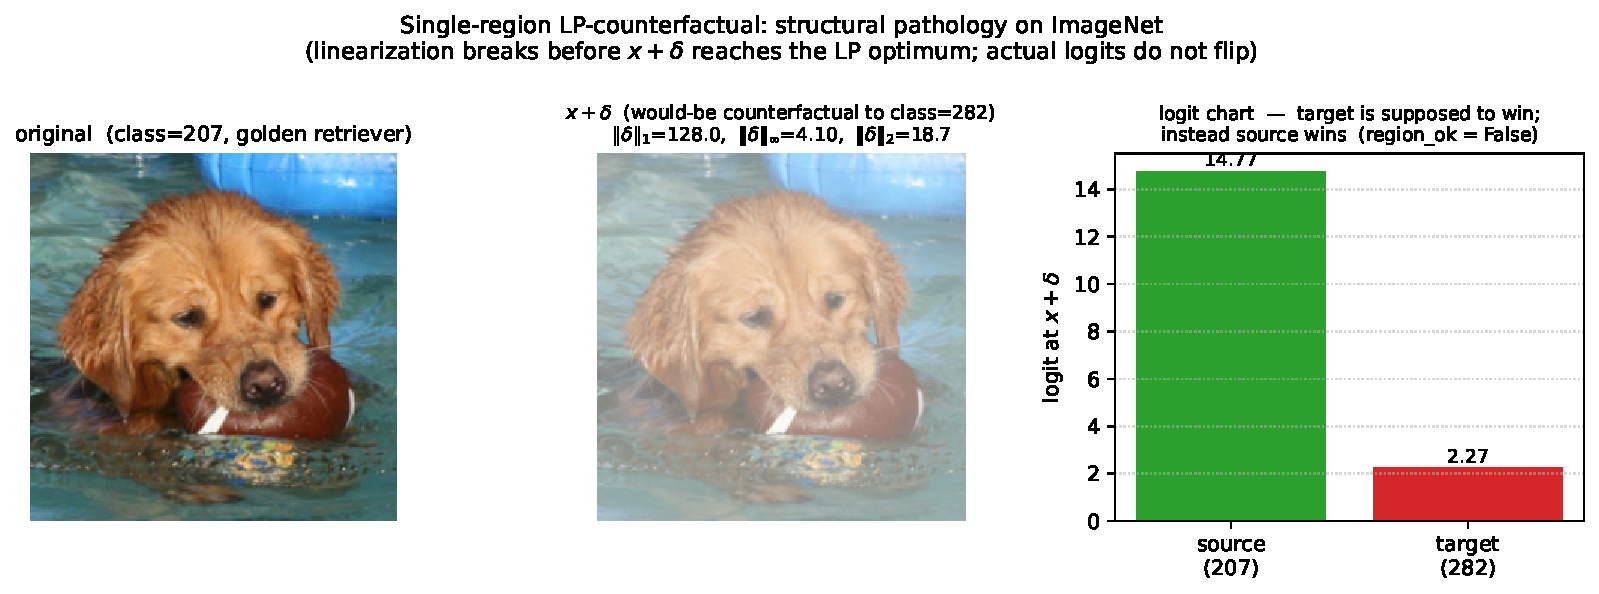
\includegraphics[width=\linewidth]{figures/lp_counterfactual_pathology.pdf}
\caption{Single-region LP-counterfactual structural failure on
DenseNet-121, source class 207 (golden retriever) $\to$ target class
282 (tiger cat). Left: original image $x$. Centre: would-be
counterfactual $x+\delta$ in ImageNet-normalised space ($\delta$
saturates $\sim25$ pixels at their per-channel pixel-space cap). Right:
at the actual (un-clamped) $x+\delta$ the source class still wins by a
large margin ($14.33$ vs.\ $1.14$); \emph{region\_ok = False}: the
region the LP solved against does not contain $x+\delta$. Every one of the
$54$ source/target pairs across the three architectures fails identically
(\emph{region\_ok} $=0/54$, Limitation~L3).}
\label{fig:lp-pathology}
\end{figure}

\WARNING{This figure predates the current revision and is the only image the
manuscript includes. Its caption asserts specific quantities --- source class
$207\to$ target $282$, logits $14.33$ vs.\ $1.14$, and ${\sim}25$ saturated
pixels --- which should be verified against the actual LP-counterfactual run
(the $\delta$ and \emph{region\_ok} records behind the $0/54$ result), and the
figure regenerated if the run has changed, before submission.}

\noindent
The LP-counterfactual is a \emph{theoretical} matrix-direction object,
not an adversarial perturbation (its magnitudes are far outside any
standard budget), and we avoid that framing deliberately. The negative
is that the matrix direction does not transfer to the model's actual
logits once it leaves the source region; a multi-region or
continuation-based reformulation is left as future work
(Section~\ref{sec:limitations}, L3).

\subsection{Teleportation drift is measured, never asserted zero}
\label{sec:study3-teleport}

\paragraph{Why it matters.}
The third negative is a claim we are careful \emph{not} to make. The
temptation in Study~1B (Section~\ref{sec:study1b}) is to enter a table zero
for the knowledge-matrix drift on the strength of the invariance theorem.
Resisting that temptation is what keeps the invariance claim of Study~1
defensible: teleportation does not verify invariance here, because its
transform is function-approximate and fails the theorem's hypothesis. We
do not assert a zero, for two reasons that compound. First, by
Theorem~\ref{thm:nogo} there is \emph{no} bound on knowledge-matrix germ
drift from function-space ($C^0$) closeness alone: two networks can be
uniformly arbitrarily close as functions yet have knowledge matrices
arbitrarily far apart at a point. Second, teleportation on
BatchNorm architectures is function-\emph{approximate}, not exact ---
every one of our $100$ teleports exceeds the $10^{-3}$ logit-drift gate
(up to $\sim10^{-1}$ on ResNet-152) because the BN running statistics are
not migrated under the change-of-basis --- so the invariance theorem's
hypothesis simply does not hold, and an asserted zero would be reporting
a number the experiment did not measure.

\paragraph{Reading.}
We therefore report knowledge-matrix drift under teleportation through
the structure of Proposition~\ref{prop:visdrift}: the visible component
is an identity equal to the logit gate and checked per pair, while the
invisible component carries no a~priori bound (Theorem~\ref{thm:nogo})
and is left unestimated here --- its empirical behaviour is exhibited on
adversarial pairs, where the gate is exact, in Study~2. This reports
only what the violated hypothesis permits, rather than asserting a zero
from a theorem whose hypothesis fails. A BN-aware teleportation that
migrates the running statistics would tighten the gate toward exactness
and is the highest-priority follow-up (Section~\ref{sec:limitations},
L1).

\paragraph{Auxiliary visualisations.}
The \texttt{km\_feature\_viz} pipeline additionally produces a
Jacobian-sensitivity heatmap, DeepDream activation-maximisation
\citep{olah2017feature}, and feature-dictionary artefacts from the same
linearisation; these are exploratory uses of $\Weff(x)$ rather than
tests of any claim in this paper, and we provide them only in the
supplementary HTML index
(\texttt{results/km-feature-viz/\_viewable/index.html}).
